%!TEX root =article.tex
\documentclass{article}

%!TEX root =article.tex
% math
\usepackage{amsmath} 
\usepackage{amssymb} 
\usepackage{amsthm}
\usepackage{color}
\usepackage{fullpage}
\usepackage{graphicx}
\usepackage{longtable}

\global\long\def\R{\mathbb{R}}


\global\long\def\modulo#1{{\left|#1\right|}}

\global\long\def\cvar{\rho}


\global\long\def\uptext{\text{U}}


\global\long\def\downtext{\text{D}}


\global\long\def\initvar#1{\bar{#1}}


\global\long\def\initstate{\initvar{\cvar}}


\global\long\def\dvar{\cvar}


\global\long\def\initdiscrete{\initvar{\dvar}}


\global\long\def\discrete#1#2{\dvar_{#1}^{#2}}


\global\long\def\pfrac#1#2{\frac{\partial#1}{\partial#2}}


\global\long\def\Dfrac#1#2{\frac{d#1}{d#2}}


\global\long\def\links{\mathcal{I}}


\global\long\def\link{i}


\global\long\def\cind{j}


\global\long\def\nlinks{N}


\global\long\def\junctions{\mathcal{J}}


\global\long\def\jns{\junctions}


\global\long\def\junction{J}


\global\long\def\jn{\junction}


\global\long\def\RS{RS}


\global\long\def\convar{u}


\global\long\def\condiscrete#1#2{\convar_{#1}^{#2}}


\global\long\def\ncontrols{M}


\global\long\def\control{\vec{\convar}}


\global\long\def\state{\vec{\dvar}}


\global\long\def\density{\cvar}


\global\long\def\densitydiscrete#1#2{\discrete{#1}{#2}}


\global\long\def\defeq{:=}


\global\long\def\vect#1{\boldsymbol{\mathbf{#1}}}


\global\long\def\Inc{\text{Inc}}


\global\long\def\Out{\text{Out}}


\global\long\def\sys{H}


\global\long\def\syseq{h}


\global\long\def\cost{C}


\global\long\def\pmat#1#2{#1_{#2}}


\global\long\def\Hx{\pmat{\sys}{\state}}


\global\long\def\Hu{\pmat{\sys}{\control}}


\global\long\def\Jx{\pmat{\cost}{\state}}


\global\long\def\Ju{\pmat{\cost}{\control}}


\global\long\def\nominal#1{#1'}


\global\long\def\evaluate#1#2{\left.#1\right|_{#2}}


\global\long\def\tind{k}


\global\long\def\xind{j}


\global\long\def\ninc{n}


\global\long\def\nout{m}


\global\long\def\jlink#1#2{\link_{#1}^{#2}}


\global\long\def\jup#1{\jn_{#1}^{\uptext}}


\global\long\def\jdown#1{\jn_{#1}^{\downtext}}


\global\long\def\tuple#1#2{\left(#1,\ldots,#2\right)}


\global\long\def\trace#1{\hat{#1}}


\global\long\def\ntime{T}


\global\long\def\juncvar#1#2#3{\vec{#1}_{#2}^{#3}}


\global\long\def\juncstate#1#2{\juncvar{\dvar}{#1}{#2}}


\global\long\def\junctrace#1#2{\juncvar{\trace{\dvar}}{#1}{#2}}


\global\long\def\junccon#1#2{\juncvar{\convar}{#1}{#2}}


\global\long\def\ssvar{W_{R}}


\global\long\def\ss#1#2#3{\ssvar\left(#1;#2,#3\right)}


\global\long\def\god{g^{G}}


\global\long\def\ramp{\convar}


\global\long\def\length{L}


\global\long\def\intrange#1#2{\left\{  #1,\ldots,#2\right\}  }


\global\long\def\degree#1{D_{#1}}


\global\long\def\demandsym{D}


\global\long\def\boundaryDemand#1#2{\demandsym_{#1}^{#2}}


\global\long\def\splitratio{\beta}


\global\long\def\barrierTerm{\epsilon}


\global\long\def\demand{\delta}


\global\long\def\rampDemand{d}


\global\long\def\supply{\sigma}


\global\long\def\ffspeed{v}


\global\long\def\congspeed{w}


\global\long\def\xdis#1{x_{#1}}


\global\long\def\fin#1#2{g_{#1,\uptext}^{#2}}


\global\long\def\fout#1#2{g_{#1,\downtext}^{#2}}


\global\long\def\framp#1#2{g_{#1,\downtext}^{#2}}

\newcommand \noiseFactor \sigma

\begin{document}

\title{Efficient methods for coordinated ramp metering using the discrete adjoint method}

%!TEX root =article.tex

% of EIGHT authors. SIX appear on the 'first-page' (for formatting
% reasons) and the remaining two appear in the \additionalauthors section.
%

\author{
Jack Reilly \and Walid Krichene \and Samitha Samaranayake \and
Maria Laura Delle Monache \and Paola Goatin \and Alexandre M. Bayen
}
\date{\today}

\maketitle

\begin{abstract}
%!TEX root = restart.tex
\begin{abstract}
The adjoint method provides a
computationally efficient means of  calculating the gradient for applications
in constrained optimization. In this  article, we consider a network of scalar
conservation laws with general topology, whose behavior is modified by a set
of control  parameters  in order to minimize a given objective function. After
discretizing the corresponding partial differential equation models  via the
Godunov scheme, we detail the computation of the gradient of the discretized
system with respect to the control parameters and  show that the complexity of
its computation scales linearly with the  number of discrete state variables
for networks of small vertex degree. The method is applied to solve the
problem of coordinated  ramp metering on freeway networks. Numerical
simulations on the I15   freeway in California demonstrate an improvement in
performance and running time compared to existing methods.
\end{abstract}

\end{abstract}

\keywords{control of discretized PDEs, network of hyperbolic conservation laws, adjoint based optimization, transportation engineering, ramp metering}

\section{Introduction}\label{sec:introduction}
%!TEX root =article.tex

\begin{itemize}
  \item why is ramp metering useful?
  \item Coordinated Ramp metering overview
  \begin{itemize}
    \item Feedback - HERO \cite{Papamichail2008}
    \item LP formulations
    \begin{itemize}
      \item ACTM \cite{gomes2006optimal}
      \item LN-CTM \cite{Muralidharana}
    \end{itemize}
    \item NL Control
    \begin{itemize}
          \item \cite{Kotsialos2004} papa
          \item cooperative, decentralized \cite{Ramon2013}
        \end{itemize}
  \end{itemize}
  \item talk about where we fit in here
  Our approach allows for nonlinear solvers to take advantage of gradient information with no relaxation of model. Additionally, it can be incorporated in an MPC framework to act as a predictive controller with feedback.
  \item introduce adjoint methods
  \begin{itemize}
    \item aircraft optimization \cite{Giles2000}
    \item air traffic control \cite{Bayen2006}
    \item jacquet stuff w/ continuous ramp metering \cite{Jacquet2005}
  \end{itemize}
  \item overview of rest of paper
  \begin{itemize}
    \item model
    \item objectives
    \item adjoint method
    \item numerical methods
    \item evaluations
    \item conclusion
  \end{itemize}
\end{itemize}

\section{Model} % (fold)
\label{sec:model}
%!TEX root =article.tex
\subsection{Network model} % (fold)
\label{sub:network_model}

% go over the sequential links, onramp, offramp assumptions.

% introduce in a continuous fashion, starting with PDE work to show that it's a rigorous reduction from PDE stuff.

We model a freeway stretch as a sequence of junctions $\junctions=\seq{\jn}{\jnidx},\jnidx=\left[0,\ldots,\nlinks -1\right]$.
Furthermore, each junction $\jn_{\jnidx}$ has an onramp with 
a maximum out flux $\rampMax_{\jnidx}$
and a merging priority $\priority_{\jnidx}$, and an offramp with
a throughput split ratio $\splitRatio_{\jnidx}$\footnote{The network parameters can all be time-dependent in the general case, but are presented as constant for simplicity.}. Connecting junctions $\jn_{\jnidx}$ and $\jn_{\jnidx+1}$ is road link $\link_{\jnidx}\in\links$, which has length $\length_\jnidx$, and the triangular fundamental diagram parameters:
free-flow speed $\vfd_{\jnidx}$, 
congestion wave speed $\wfd_{\jnidx}$, 
critical density $\pcfd_{\jnidx}$, 
max density $\pmfd_{\jnidx}$, and
max flux $\fmfd_{\jnidx}$. The choice of a triangular fundamental diagram is supported by empirical evidence on freeway networks of a distinct ``free-flow'' phase with constant velocity as a function of density, and a congestion phase with decreasing capacity as a function of density. Figure~\ref{fig:freeway-network} summarizes the network topology and parameters.

\begin{figure}
\centering

\includegraphics[width=.25\columnwidth]{figures/placeholder}
\caption{Freeway stretch network and parameters}
\label{fig:freeway-network}
\end{figure}

\subsection{Dynamics} % (fold)
\label{sub:dynamics}

Since we wish to have numerical stability in our model dynamics, we use a macroscopic traffic-flow model, derived from partial differential equations.
We use a first-order LWR \cite{lighthill1955kinematic,richards1956shock} network model developed in~\cite{Monache2013}, which is particularly suitable for freeway control and can be seen as an extension of the model in~\cite{garavello2006traffic}. The model in~\cite{Monache2013} is employed for its strong boundary conditions on the onramps to ensure all flux demand passes through the network~\cite{strub2006weak} and ability to accurately model $2\times2$ junctions without blocking onramp flux.

In order to simulate the model or use it within an optimization framework, we first discretize the model using the Godunov scheme~\cite{godunov1959}, as detailed in~\cite{Monache2013}. The initial conditions of the model are set by specifying an initial density $\po$ (vehicles per unit length) for all links and an initial queue length $\lo$ (vehicles) for all onramps. The boundary conditions are specified as ramp flux demands $\rampBC$ for all ramps and all time steps, noting that the upstream mainline source is modeled as an onramp.

The system of equations for the discretized system is given in Equation~\eqref{eqn:system-of-equations}, for a given link $i \in \left[0,\ldots,\horizon\right]$ and time step $k \in \left[0,\ldots,\horizon\right]$.

\begin{equation}
\begin{aligned}
\label{eqn:system-of-equations}
% density
\idx{\density}{i}{k} & = & &
\idx{\density}{i}{k-1} + \frac{\dt}{\length_i} \left(\idx{\fIn}{i}{k-1} - \idx{\fOut}{i}{k-1}\right)
\\
% queue
\idx{\queue}{i}{k} & = & &
\idx{\queue}{i}{k-1} + \dt \left(\idx{\rampBC}{i}{k-1} - \idx{\fRamp}{i}{k-1}\right) \\
% demand
\idx{\demand}{i}{k} & = & &
\min\left( \fmfd_i, \vfd_i \idx{\density}{i}{k} \right)
\\
% supply
\idx{\supply}{i}{k} & = & &
\min\left(\fmfd_i, \wfd \left( \pmfd_i - \idx{\density}{i}{k} \right)\right)
\\
% ramp demand
\idx{\rampDemand}{i}{k} & = & &
\min\left( \rampMax_i, \idx{\queue}{i}{k} / \dt \right)
\\
% flux in
\footnotemark
\idx{\fIn}{i}{k} & = & &
\min\left( \splitRatio_{i-1} \idx{\demand}{i-1}{k} + \idx{\rampDemand}{i}{k}, \idx{\supply}{i}{k} \right)
\\
% flux out
\idx{\fOut}{i}{k} & = & &
\begin{cases}
% case 1
\idx{\demand}{i}{k} &
\frac{\idx{\supply}{i+1}{k}\priority_{i+1}}{1 + \priority_{i+1}} \ge \idx{\demand}{i}{k}\splitRatio_{i+1}{k} \\
% case 2
\left(\idx{\fIn}{i+1}{k} - \idx{\rampDemand}{i_1}{k}\right) / \splitRatio_{i +1} & 
\frac{\idx{\supply}{i+1}{k}}{1 + \priority_{i+1}} \ge \idx{\rampDemand}{i}{k} \\
% case 3
\frac{\idx{\supply}{i+1}{k}\priority_{i+1}}{\left(1 + \priority_{i+1}\right)\splitRatio_{i+1}{k}} &
\text{otherwise}
\end{cases}
\\
% ramp flux
\idx{\fRamp}{i}{k} & = & &
\idx{\fIn}{i}{k} - \splitRatio_{i} \idx{\fOut}{i-1}{k}
\end{aligned}
\end{equation}

\footnotetext{This is a simplification of~\cite{Monache2013} for the case when the ramp empties on a time step, with minimal effect on numerical results.}

The intermediate variables (those used to calculate the states variables, $\density$ and $\queue$) represent the following values; $\demand$, the demand, is the amount of flux that a link can send downstream in a time step; $\supply$, the supply, is the amount of flux that a link can receive; $\rampDemand$, the ramp demand, is the amount of flux that an onramp can send; $\fIn/\fOut$ is the flux that enters/exits upstream/downstream of a link; $\fRamp$ is the flux that exits an onramp.

\paragraph*{Control parameters} % (fold)
\label{sub:control_parameters}

% The $\sysMat$ system in Section~\ref{sub:dynamics} expresses the relationships of all state variables, which can be solved to give a forward simulation of the system. 
In order to affect the system externally, we must introduce some control parameters. We denote control parameters with $\control$. One method of control, known as variable speed limits~\cite{Muralidharan2009}, would set $\control$ as the free-flow velocity of the fundamental diagrams. State estimation problems can be posed in this fashion by letting $\control$ be the initial conditions, and searching for an initial condition that evolves to a known final state~\cite{Jacquet}. Ramp metering sets $\control$ as the maximum outflow from onramps. 

\jdrcomment{below maybe moved to ramp metering specific section}
More precisely, we say $\idx{\control}{i}{k}$ sets an upper limit on the flux out of onramp $i$ at time $k$. For the case of ramp metering, we modify the $\rampDemand$ equation in~\eqref{eqn:system-of-equations} to account for this new parameter:

\begin{equation}
\label{eqn:modified-ramp-demand}
\idx{\rampDemand}{i}{k} = 
\min\left( \idx{\control}{i}{k}, \rampMax_i, \idx{\queue}{i}{k} / \dt \right)
\end{equation}

\paragraph*{System matrix}

By taking the dynamics conditions in Equation~\eqref{eqn:system-of-equations}, the initial and boundary conditions, and subtracting the right hand side of each equation in the system, we can construct the system matrix $\sysMat \left( \state, \control \right) = 0$, where $\state\in\Rbb^{\nState}$ ($\nState=|x|$) is the entire state vector, ordered first by time step, then by variable type (e.g. $\density, \queue, \demand,$ etc), and finally by link. The control vector $\control\in\Rbb^{\nControl}$ ($\nControl = |\control|$) is ordered similarly. More details about the ordering and its effect on the efficiency of gradient computation is given in Section~\ref{sub:efficient_solution_of_system_via_depth_first_search_system_solution}. The system of equations can be solved in linear time via forward-substitution (a result of the system being triangular), similar to other first-order network models such as the cell transmission model~\cite{daganzo1995cell}. The variable dependencies are graphically depicted in Figure~\ref{fig:variable-dependencies}.

\begin{figure}
\centering
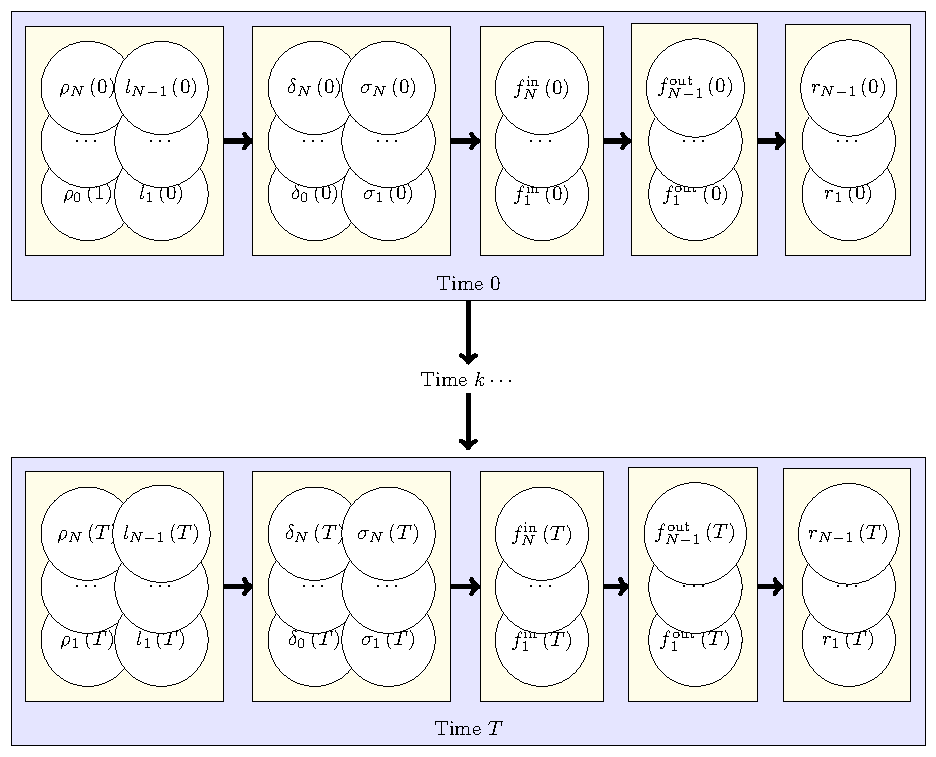
\includegraphics[width=.75\columnwidth]{oldPaper/triangletikzpdf}
\caption{Forward system variable dependencies. Ordering in this fashion leads to a lower-triangular system, which is efficient to solve.}
\label{fig:variable-dependencies}
\end{figure}


% subsection control_parameters_for_ramp_metering (end)

\subsection{Cost function} % (fold)
\label{sub:minimzing_total_travel_time}
This part should be short. Talk about modeling the optimization problem, with dynamics as the constraints. 

Then, discuss the extensibility of the formulation to other problems

\begin{itemize}
    \item State estimation
    \item Variable Speed limits
    \item Rerouting (probably cite some of my previous work)
\end{itemize}


% section minimzing_total_travel_time (end)

% section model (end)

\section{Minimzing total travel time} % (fold)
\label{sec:minimzing_total_travel_time}
This part should be short. Talk about modeling the optimization problem, with dynamics as the constraints. 

Then, discuss the extensibility of the formulation to other problems

\begin{itemize}
    \item State estimation
    \item Variable Speed limits
    \item Rerouting (probably cite some of my previous work)
\end{itemize}


% section minimzing_total_travel_time (end)

\section{Solving the discrete adjoint system} % (fold)
\label{sec:solving_the_discrete_adjoint_system}

\section{Adjoint based flow optimization\label{sec:Adjoint-method}}


\subsection{Optimal control problem formulation\label{par:Optimization-Problem}}

In addition to our governing equations $\sys\left(\state,\control\right)=0$,
we also introduce a cost function $\cost$, which we assume to be
in $C^{2}$:

\begin{eqnarray*}
	\cost: & \mathbb{R}^{\nlinks T}\times\mathbb{R}^{\ncontrols T} & \rightarrow\mathbb{R}\\
	& \left(\state,\control\right) & \mapsto\cost\left(\state,\control\right)
\end{eqnarray*}


which returns a scalar that serves as a metric of performance of the
state and control values of the system. We wish to minimize the quantity
$\cost$ over the set of control parameters $\control$, while constraining
the state of the system to satisfy the governing equations $\sys\left(\state,\control\right)=0$,
which is, again, the concatenated version of~\eqref{eq:main-ge} or~\eqref{eq:syseq-god}.
We summarize this with the following optimization problem:

\begin{eqnarray}
	\underset{\control}{\min} & \cost\left(\state,\control\right)\nonumber \\
	\text{subject to:} & \sys\left(\state,\control\right)=0\label{eq:op-problem}
\end{eqnarray}


Both the cost function and governing equations may be non-convex in
this problem.


\subsection{Calculating the gradient\label{par:Calculating-the-gradient}}

We wish to use gradient information in order to find control values
$\control^{*}$ that give locally optimal costs $\cost^{*}=\cost\left(\state\left(\control^{*}\right),\control^{*}\right)$.
Since there may exist many local minima for this optimization problem~\eqref{eq:op-problem}
(which is non-convex in general), gradient\emph{ }methods do not guarantee
global optimality of $\control^{*}$\emph{. }Still, nonlinear optimization
methods such as interior point optimization utilize gradient information
to improve performance~\cite{Andreas2005}.

In a descent algorithm, the optimization procedure will have to descend
a cost function, by coupling the gradient, which, at a nominal point
$\left(\nominal{\state},\nominal{\control}\right)$ is given by:

\begin{equation}
	d_{\control}\cost\left(\nominal{\state},\nominal{\control}\right)=\evaluate{\pfrac{\cost\text{\ensuremath{\left(\state,\control\right)}}}{\state}}{\nominal{\state},\nominal{\control}}\Dfrac{\state}{\control}+\evaluate{\pfrac{\cost\text{\ensuremath{\left(\state,\control\right)}}}{\control}}{\nominal{\state},\nominal{\control}}\label{eq:j-v}
\end{equation}


The main difficulty is to compute the term $\Dfrac{\state}{\control}$.
Next we take advantage of the fact that the derivative of $H\left(\state,\control\right)$
with respect to $\control$ is equal to zero along trajectories of
the system:

\begin{equation}
	d_{\control}\sys\left(\nominal{\state},\nominal{\control}\right)=\evaluate{\pfrac{\sys\text{\ensuremath{\left(\state,\control\right)}}}{\state}}{\nominal{\state},\nominal{\control}}\Dfrac{\state}{\control}+\evaluate{\pfrac{\sys\text{\ensuremath{\left(\state,\control\right)}}}{\control}}{\nominal{\state},\nominal{\control}}=0\label{eq:h-v}
\end{equation}


The partial derivative terms, $\Hx\in\mathbb{R}^{\nlinks\ntime\times\nlinks\ntime}$,
$\Hu\in\mathbb{R}^{\nlinks\ntime\times\ncontrols\ntime}$, $\Jx\in\mathbb{R}^{\nlinks\ntime}$,
and $\Ju\in\mathbb{R}^{\ncontrols\ntime}$, can all be evaluated (more
details provided in Section~\ref{sub:Evaluating--and}) and then
treated as constant matrices. Thus, in order to evaluate $d_{\control}\cost\left(\nominal{\state},\nominal{\control}\right)\in\mathbb{R}^{\ncontrols\ntime}$,
we must solve a coupled system of matrix equations.
\begin{note}
	In~\eqref{eq:h-v}, $\Hx$ and $\Hu$ might not necessarily by defined,
	either because $f$ itself is not smooth (note that we took $f$ to
	be $C^{2}$ to avoid this problem), and/or because $\god$ is not
	smooth. The derivations below are valid when the partials $\Hx$ and
	$\Hu$ can indeed be taken. There are several settings in which the
	conditions for differentiability are satisfied, see in particular~\cite{Gugat2005,Flasskamp2012}.
\end{note}

\paragraph{Forward system.\label{par:Forward-system}}

If we solve for $\Dfrac{\state}{\control}\in\mathbb{R}^{\nlinks\ntime\times\ncontrols\ntime}$
in~\eqref{eq:h-v}, which we call the \emph{forward system}:

\[
	\Hx\Dfrac{\state}{\control}=-\Hu,
\]


then we can substitute the solved value for $\Dfrac{\state}{\control}$
into~\eqref{eq:j-v} to obtain the full expression for the gradient.
Section~\ref{sub:Evaluating--and} below gives details on the invertibility
of $\Hx$, guaranteeing a solution for $\Dfrac{\state}{\control}$.


\paragraph{Adjoint system.\label{par:Adjoint-system}}

Instead of evaluating $\Dfrac{\state}{\control}$ directly, the adjoint
method instead solves the following system, called the adjoint system,
for a new unknown variable $\lambda\in\mathbb{R}^{\nlinks\ntime}$
(called the adjoint variable):

\begin{equation}
	\Hx^{T}\lambda=-\Jx^{T}\label{eq:adjoint}
\end{equation}
Then the expression for the gradient becomes:

\begin{equation}
	d_{\control}\cost\left(\nominal{\state},\nominal{\control}\right)=\lambda^{T}\Hu+\Ju\label{eq:adjoint-grad}
\end{equation}
We define $\degree{\state}$ to be the maximum junction degree on
the network:

\begin{equation}
	\degree{\state}=\max_{\jn\in\jns}\left(\ninc_{\jn}+\nout_{\jn}\right),\label{eq:dx}
\end{equation}
and also define $\degree{\control}$ to be the maximum number of constraints
that a single control variable appears in, which is equivalent to:

\begin{equation}
	\degree{\control}=\max_{\condiscrete{}{}\in\control}\sum_{\jn\in\jns:\condiscrete{}{}\in\junccon{\jn}{\tind}}\left(\ninc_{\jn}+\nout_{\jn}\right)\label{eq:dv}
\end{equation}


Note that $\left\{ \convar\in\junccon{\jn}{\tind}:\jn\in\jns\right\} $
is a $\tind$-dependent set. By convention, junctions are either actuated
or not, so there is no dependency on $\tind$, i.e. if $\exists\tind$
s.t. $\convar\in\junccon{\jn}{\tind}$, then $\forall\tind$, $\convar\in\junccon{\jn}{\tind}$.

Using these definitions, we show later in Section~\ref{sub:Complexity-of-solving}
how the complexity of computing the gradient is reduced from $O(\degree{\state}\nlinks\ncontrols\ntime^{2})$
to $O(\ntime\left(\degree{\state}\nlinks+\degree{\control}\ncontrols\right))$
by considering the adjoint method over the forward method.

A graphical depiction of $D_{\state}$ and $D_{\control}$ are given
in Figure~\ref{fig:Depicting--and}
\begin{figure}
	\begin{centering}
		\subfloat[\label{fig:genneta}]{\begin{centering}
			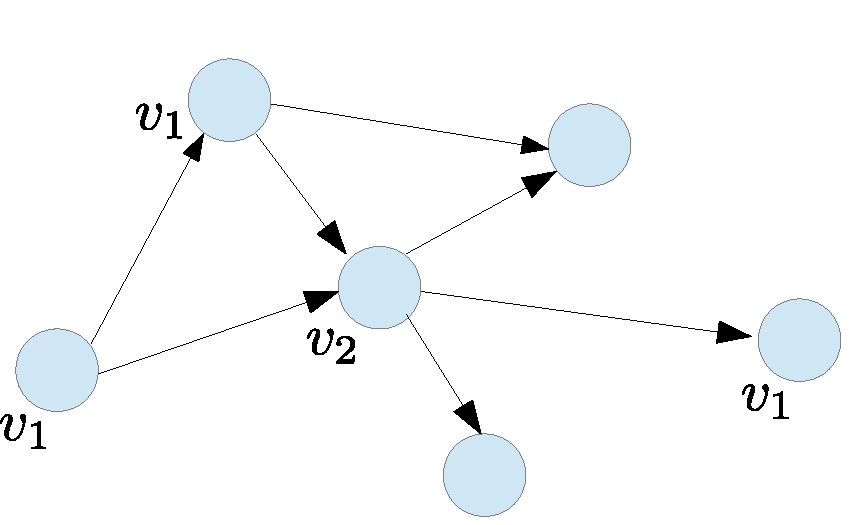
\includegraphics[width=0.33\columnwidth]{figs-gen/gen-net}
			\par\end{centering}
						
			}\subfloat[\label{fig:gennetb}]{\begin{centering}
			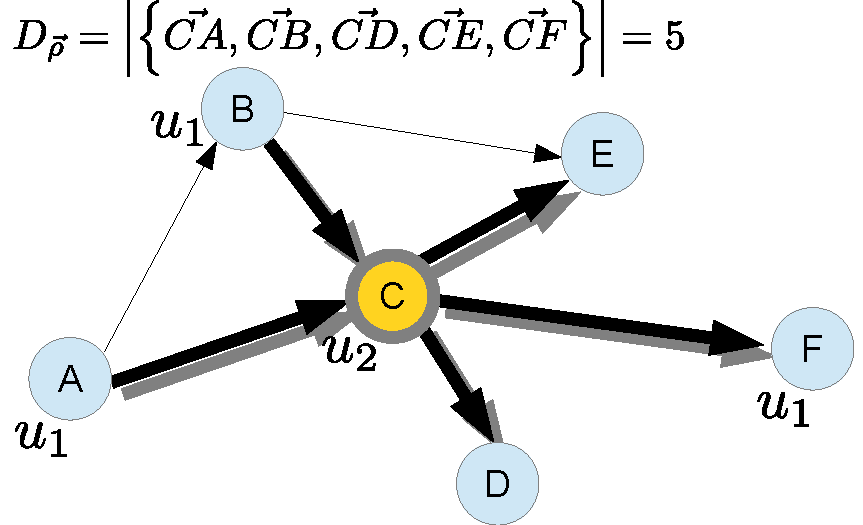
\includegraphics[width=0.33\columnwidth]{figs-gen/gen-net-dx}
			\par\end{centering}
						
			}\subfloat[\label{fig:gennetc}]{\begin{centering}
			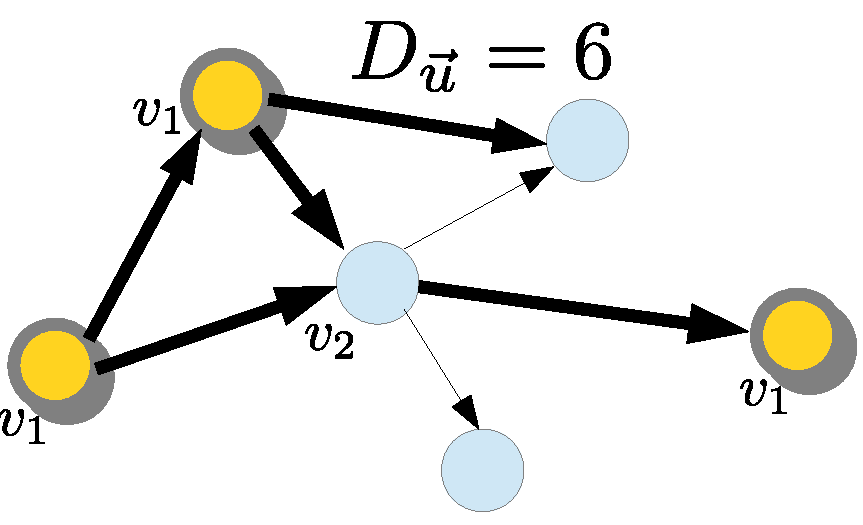
\includegraphics[width=0.33\columnwidth]{figs-gen/gen-net-dv}
			\par\end{centering}
						
		}
		\par\end{centering}
				
		\caption{Depiction of $D_{\state}$ and $D_{v}$ for an arbitrary graph. Figure~\ref{fig:genneta}
			shows the underlying graphical structure for an arbitrary PDE network.
			Some control parameter $\convar_{1}$ has influence over junctions
			$A$, $B$, and $F$, while another control parameter $\convar_{2}$
			has influence over only junction $C$. Figure~\ref{fig:gennetb}
			depicts the center junction having the largest number of connecting
			edges, thus giving $D_{\state}=5$. Figure~\ref{fig:gennetc} shows
			that control parameter $\convar_{1}$ influences three junctions with
			sum of junctions degrees equal to six, which is maximal over the other
			control parameter $\convar_{2}$. leading to the result $D_{\control}=6$.
			Note that in Figure~\ref{fig:gennetc}, the link going from junction
			$A$ to junction $B$ is counted twice: once as an outgoing link $\vec{AB}$
			and once as in incoming link $\vec{BA}$.\label{fig:Depicting--and}}
		\end{figure}
		.Freeway networks are usually considered to have topologies that are
		nearly planar, leading to junctions degrees which typically do not
		exceed 3 or 4, regardless of the total number of links. Also, from
		the locality argument for control variables in Section~(\ref{sec:State,-control,-and}),
		a single control variable's influence over state variables will not
		grow with the size of the network. Since the $\degree{\state}$ and
		$\degree{\control}$ typically do not grow with $\nlinks\ntime$ or
		$\ncontrols\ntime$ for freeway networks, the complexity of evaluating
		the gradient for such networks can be considered linear for the adjoint
		method.
				
				
		\subsection{Evaluating the partial derivatives\label{sub:Evaluating--and}}
				
		While no assumptions are made about the sparsity of the cost function
		$\cost$, the networked-structure of the PDE system and the Godunov
		discretization scheme allows us to say more about the structure and
		sparsity of $\Hx$ and $\Hu$.
				
				
		\paragraph{Partial derivative expressions.}
				
		Given that the governing equations require the evaluation of a Riemann
		solver at each step, we detail some of the necessary computational
		steps in evaluating the $\Hx$ and $\Hu$ matrices. 
				
		If we consider a particular governing equation $\syseq_{\link}^{\tind}\left(\state,\control\right)=0$,
		then we may determine the partial term with respect to $\discrete jl\in\state$
		by applying the chain rule:
				
		\begin{align}
			\pfrac{\syseq_{\link}^{\tind}}{\discrete jl}=\pfrac{\discrete{\link}{\tind}}{\discrete jl}-\pfrac{\discrete{\link}{\tind-1}}{\discrete jl} & +\frac{\Delta t}{L_{i}}f'\left(\RS_{\jdown{\link}}\left(\juncstate{\jdown{\link}}{\tind-1},\junccon{\jdown{\link}}{\tind-1}\right)_{\link}\right)\pfrac{}{\discrete jl}\left(\RS_{\jdown{\link}}\left(\juncstate{\jdown{\link}}{\tind-1},\junccon{\jdown{\link}}{\tind-1}\right)_{\link}\right)\label{eq:dhdufull} \\
			                                                                                                                                           & -\frac{\Delta t}{L_{i}}f'\left(\RS_{\jup{\link}}\left(\juncstate{\jup{\link}}{\tind-1},\junccon{\jup{\link}}{\tind-1}\right)_{\link}\right)\pfrac{}{\discrete jl}\left(\RS_{\jup{\link}}\left(\juncstate{\jup{\link}}{\tind-1},\junccon{\jup{\link}}{\tind-1}\right)_{\link}\right)\nonumber                       
		\end{align}
				
				
		or if we consider the composed Riemann flux solver $\god_{\jn}$ in~\eqref{eq:god-jn}:
				
		\begin{equation}
			\pfrac{\syseq_{\link}^{\tind}}{\discrete jl}=\pfrac{\discrete{\link}{\tind}}{\discrete jl}-\pfrac{\discrete{\link}{\tind-1}}{\discrete jl}+\frac{\Delta t}{L_{i}}\left(\pfrac{}{\discrete jl}\left(\god_{\jdown{\link}}\left(\juncstate{\jdown{\link}}{\tind-1},\junccon{\jdown{\link}}{\tind-1}\right)\right)_{\link}-\pfrac{}{\discrete jl}\left(\god_{\jup{\link}}\left(\juncstate{\jup{\link}}{\tind-1},\junccon{\jup{\link}}{\tind-1}\right)\right)_{\link}\right)\label{eq:dhdugod}
		\end{equation}
				
				
		A diagram of the structure of the $\Hx$ matrix is given in Figure~(\ref{fig:partial-ordering}).
		\begin{figure}
			\subfloat[\label{fig:partial-ordering}Ordering of the partial derivative terms.
				Constraints and state variables are clustered first by time, and then
				by cell index.]{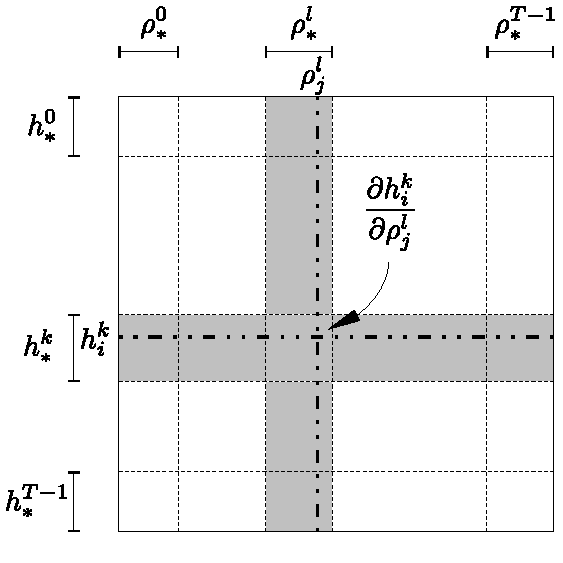
\includegraphics[width=0.45\columnwidth]{figs-gen/dstate}
												
						}\texttt{\hfill{}}\subfloat[\label{fig:sparsity-diagram}Sparsity structure of the $\Hx$ matrix.
				Besides the diagonal blocks, which are identity matrices, blocks where
				$l\neq\tind-1$ are zero.]{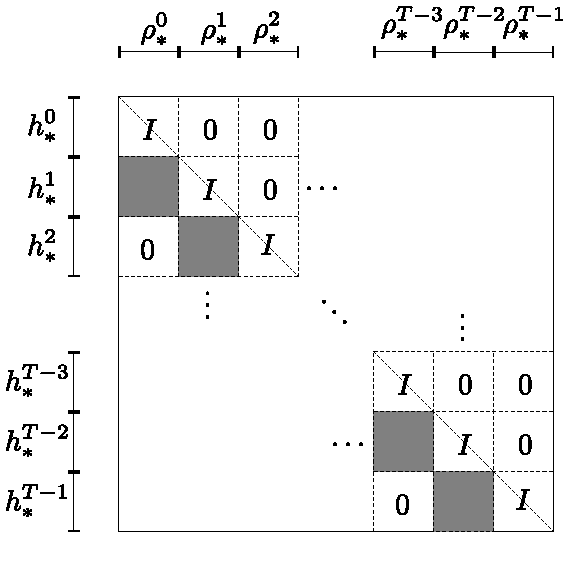
\includegraphics[width=0.45\columnwidth]{figs-gen/sparsity-two}
												
						\texttt{}
												
					}
										
					\caption{Structure of the $\Hx$ matrix.}
										
										
				\end{figure}
				Similarly for $H_{v}$, we take a control parameter $\condiscrete jl\in\control$,
				and derive the expression:
								
				\begin{align}
					\pfrac{\syseq_{\link}^{\tind}}{\condiscrete jl}= & +\frac{\Delta t}{L_{i}}f'\left(\RS_{\jdown{\link}}\left(\juncstate{\jdown{\link}}{\tind-1},\junccon{\jdown{\link}}{\tind-1}\right)_{\link}\right)\pfrac{}{\condiscrete jl}\left(\RS_{\jdown{\link}}\left(\juncstate{\jdown{\link}}{\tind-1},\junccon{\jdown{\link}}{\tind-1}\right)_{\link}\right)\label{eq:dhdvfull} \\
					                                                 & -\frac{\Delta t}{L_{i}}f'\left(\RS_{\jup{\link}}\left(\juncstate{\jup{\link}}{\tind-1},\junccon{\jup{\link}}{\tind-1}\right)_{\link}\right)\pfrac{}{\condiscrete jl}\left(\RS_{\jup{\link}}\left(\juncstate{\jup{\link}}{\tind-1},\junccon{\jup{\link}}{\tind-1}\right)_{\link}\right)\nonumber                       
				\end{align}
								
								
				or for the composed Godunov junction flux solver $\god_{\jn}$:
								
				\begin{equation}
					\pfrac{\syseq_{\link}^{\tind}}{\condiscrete jl}=\frac{\Delta t}{L_{i}}\left(\pfrac{}{\condiscrete jl}\left(\god_{\jdown{\link}}\left(\juncstate{\jdown{\link}}{\tind-1},\junccon{\jdown{\link}}{\tind-1}\right)\right)_{\link}-\pfrac{}{\condiscrete jl}\left(\god_{\jup{\link}}\left(\juncstate{\jup{\link}}{\tind-1},\junccon{\jup{\link}}{\tind-1}\right)\right)_{\link}\right)\label{eqdhdvgod}
				\end{equation}
								
								
				Analyzing~\eqref{eq:dhdufull}, the only partial terms that are not
				trivial to compute are $\pfrac{}{\discrete jl}\left(\RS_{\jdown{\link}}\left(\juncstate{\jdown{\link}}{\tind-1},\junccon{\jdown{\link}}{\tind-1}\right)_{\link}\right)$
				and $\pfrac{}{\discrete jl}\left(\RS_{\jup{\link}}\left(\juncstate{\jup{\link}}{\tind-1},\junccon{\jup{\link}}{\tind-1}\right)_{\link}\right)$.
				Similarly for~\eqref{eq:dhdvfull}, the only nontrivial terms are
				$\pfrac{}{\condiscrete jl}\left(\RS_{\jdown{\link}}\left(\juncstate{\jdown{\link}}{\tind-1},\junccon{\jdown{\link}}{\tind-1}\right)_{\link}\right)$
				and $\pfrac{}{\condiscrete jl}\left(\RS_{\jup{\link}}\left(\juncstate{\jup{\link}}{\tind-1},\junccon{\jup{\link}}{\tind-1}\right)_{\link}\right)$.
				Once one obtains the solutions to these partial terms, then one can
				construct the full $\Hx$ and $\Hu$ matrices and use~\eqref{eq:adjoint}
				and~\eqref{eq:adjoint-grad} to obtain the gradient value.
								
				As these expressions are written for a general scalar conservation
				law, the only steps in computing the gradient that are specific to
				a particular conservation law and Riemann solver are computing the
				derivative of the flux function $f$ and the partial derivative terms
				just discussed. These expressions are explicitly calculated for the
				problem of optimal ramp metering in Section~(\ref{sec:Applications-to-Optimal}).
								
								
				\subsection{Complexity of solving gradient via forward method vs. adjoint method\label{sub:Complexity-of-solving}}
								
								
				\paragraph{Structure and sparsity.\label{par:Structure-and-sparsity}}
								
				We can show the lower-triangular structure and invertibility of $\Hx$
				by examining~\eqref{eq:init-ge} and~\eqref{eq:main-ge}. For $\tind\in\intrange 1{\ntime-1}$,
				we have that $\syseq_{\link}^{\tind}$ is only a function of $\discrete{\link}{\tind}$
				and of the state variables from the previous time-step $\tind-1$.
				Thus, based on our ordering scheme in Section~\ref{sec:State,-control,-and}
				of ordering variables by increasing time-step and ordering constraints
				by corresponding variable, we know for $\Hx$, diagonal terms are
				always $1$ and all upper-triangular terms must be zero (since those
				terms correspond to constraints with a dependence of \emph{future}
				values). These two conditions demonstrate both that $\Hx$ is lower-triangular
				and is also invertible due to the identity matrix block-diagonal terms.
								
				Additionally, if we consider taking partial derivatives with respect
				to the variable $\discrete jl$, then we can deduce from Equation~\eqref{eq:main-ge}
				that all partial terms will be zero except for the diagonal term,
				and those terms involving constraints at time $j+1$ with links connecting
				to the downstream and upstream junctions $\jdown j$ and $\jup j$
				respectively. To summarize, $\Hx$ matrices for systems described
				in Section~\ref{sec:State,-control,-and} will be square, invertible,
				lower-triangular and each column will have a maximum cardinality equal
				to $\degree{\state}$ in~\eqref{eq:dx}. The sparsity structure of
				$\Hx$ is depicted in Figure~(\ref{fig:sparsity-diagram}).
								
				Using the same line of argument for maximum cardinality in $\Hx$,
				we can bound the maximum cardinality of each column of $\Hu$. Taking
				a single control variable $\condiscrete jl$, the variable can only
				appear in constraints at time-step $j+1$ that correspond to a link
				that connects to a junction $\jn$ such that $\condiscrete jl\in\junccon{\jn}{l+1}$.
				These conditions give us the expression for $\degree{\control}$ in~\eqref{eq:dv},
				or the maximum cardinality over all columns in $\Hu$.
								
				If we only consider the lower triangular form of $\Hx$, then the
				complexity of solving for the gradient using the forward system is
				$O(\left(\nlinks\ntime\right)^{2}\ncontrols\ntime)$, where the dominating
				term comes from solving~\eqref{eq:j-v}, which requires the solution
				of $\ncontrols\ntime$ separate $\nlinks\ntime\times\nlinks\ntime$
				lower-triangular systems. The lower-triangular system allows for forward
				substitution, we can be solved in $O(\left(\nlinks\ntime\right)^{2})$
				steps, giving the overall complexity $O(\left(\nlinks\ntime\right)^{2}\ncontrols\ntime)$.
				The complexity of computing the gradient via the adjoint method is
				$O(\left(\nlinks\ntime\right)^{2}+\left(\nlinks\ntime\right)\left(\ncontrols\ntime\right))$,
				which is certainly more efficient than the forward-method, as long
				as $\ncontrols\ntime>1$. The efficiency is gained by considering
				that~\eqref{eq:adjoint} only requires the solution of a single $\nlinks\ntime\times\nlinks\ntime$
				\emph{upper}-triangular system (via backward-substitution), followed
				by the multiplication of $\lambda^{T}H_{v}$, an $\nlinks\ntime\times\nlinks\ntime$
				and an $\nlinks\ntime\times\ncontrols\ntime$ matrix in~\eqref{eq:adjoint-grad},
				with a complexity of $O(\left(\nlinks\ntime\right)^{2}+\left(\nlinks\ntime\right)\left(\ncontrols\ntime\right))$.
								
				For the adjoint method, this complexity can be improved upon by considering
				the sparsity of the $\Hx$ and $\Hu$ matrices, as detailed in Section~\ref{par:Structure-and-sparsity}.
				For the backward-substitution step, each entry in the $\lambda$ vector
				is solved by \emph{at most} $\degree{\state}$ multiplications, and
				thus the complexity of solving~\eqref{eq:adjoint} is reduced to
				$O(\degree{\state}\nlinks\ntime)$. Similarly, for the matrix multiplication
				of $\lambda^{T}H_{v}$, while $\lambda$ is not necessarily sparse,
				we know that each entry in the resulting vector requires at most $\degree{\control}$
				multiplications, giving a complexity of $O(\degree{\control}\ncontrols\ntime)$. 
				\begin{prop}
					\textup{The total complexity for the adjoint method on a scalar hyperbolic
						network of PDEs is }$O(\ntime\left(\degree{\state}\nlinks+\degree{\control}\ncontrols\right))$.\end{prop}
				


% section solving_the_adjoint_system (end)

\section{Numerical methods} % (fold)
\label{sec:numerical_methods}

\section{Numerical results for model predictive control simulations\label{sec:Numerical-results-for}}

To demonstrate the effectiveness of using the adjoint ramp metering
method to compute gradients, we implemented the algorithm in MATLAB.
The algorithm can then be used as a gradient computation subroutine
inside any descent-method optimization solver that takes advantage
of first-order gradient information. Our implementation makes use
of the open-source \emph{IpOpt} solver~\cite{Andreas2005}. To serve
as comparisons, three other methods were implemented:
\begin{enumerate}
\item No control: the metering rate is set to 1 on all onramps at all times.
\item Alinea~\cite{Papageorgiou1991}: a popular, feedback-based ramp metering
algorithm. Alinea is computationally efficient and decentralized,
making it a popular choice for large networks, but does not take estimated
boundary flow data as input. Since Alinea has a number of tuning parameters,
we perform a \emph{modified} grid-search technique over the different
parameters that scales linearly with the number of onramps, and select
the best-performing parameters. A \emph{full} grid-search approach
scales exponentially with the number of onramps, rendering it infeasible
for moderate-size freeway networks.
\item Descent method without gradient information: in the absence of gradient
information, the descent-method solver will estimate the gradient
by perturbing control parameters and recomputing the objective function.
\end{enumerate}
The descent method proved to be infeasible for even small, synthetic
networks. Running ramp metering on even a network of 4 links over
6 time-steps for only 5 gradient steps took well over 4 minutes. Already,
the method cannot be used in real-time for freeway networks. The comparison
of running times with and without gradient computations is given in
Figure~\ref{fig:Running-time-of}. We do not consider the method
without gradient computations in further results, due to the impractically
large running times, which only becomes worse as the problem scales
to larger networks and time horizons.
\begin{figure}
\begin{centering}
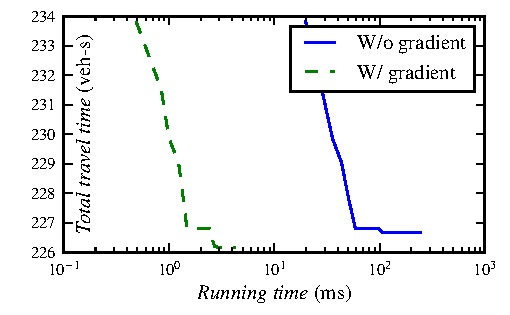
\includegraphics[width=0.65\columnwidth]{images/itergrad}
\par\end{centering}

\caption{Running time of metering algorithm with and without gradient computations.
Network consists of 4 links and 6 time-steps with synthetic boundary
flux data. The method using gradient computations via the adjoint
method converged well before the first step was completed with the
method that used perturbations to compute the gradient.\label{fig:Running-time-of}}
\end{figure}



\subsection{Network\label{sub:Network}}

As input into the optimization problem, we constructed a model of
a 19.4 miles
 stretch of the I15 South freeway in San Diego,
California between San Marcos and Mira Mesa.The network has $\nlinks=$
125
 links, $\ncontrols=$9
 onramps,
with boundary data specified for $\ntime=$ 1800 time-steps,
for a time horizon of 120.0 minutes
 given $\Delta t=$ 4 seconds
.
The network is shown in Figure~\ref{fig:Model-of-section}.
\begin{figure}
\begin{centering}
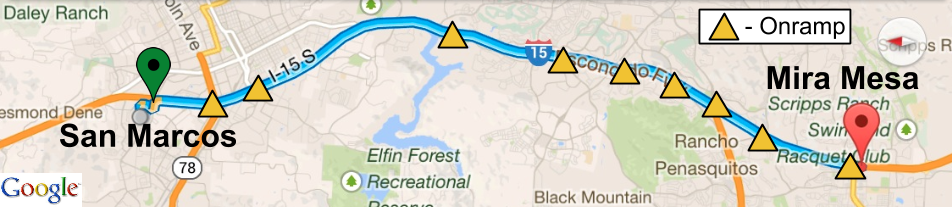
\includegraphics[width=0.7\columnwidth]{images/map}
\par\end{centering}

\caption{Model of section of I15 South in San Diego, California. The freeway
section spanning~19.4 miles was split into~125 links with 9 onramps.\label{fig:Model-of-section}}
\end{figure}


Link length data was obtained using the Scenario Editor software developed
as part of the Connected Corridors project, a collaboration between
UC Berkeley and PATH research institute in Berkeley, California.
Fundamental diagram parameters, split ratios, and boundary data were
also obtained using calibration techniques developed by Connected
Corridors. Densities resulting in free-flow speeds were chosen as
initial conditions on the mainline and onramps. The data used in calibration
was taken from PeMS sensor data during a morning rush hour period,
scaled to generate congested conditions. The input data was chosen
to demonstrate the effectiveness of the adjoint ramp metering method
in a real-world setting. A profile of the mainline and onramps during
a forward simulation of the network is shown in Figure~\ref{fig:Density-and-queue}
under the described boundary conditions.
\begin{figure}
\subfloat[Density profile. The units are the ratio of a link's vehicle density
to a link's critical density. Values less than 1 represent free flow,
while values greater than 1 represent congestion.\label{fig:Density-profile.}]{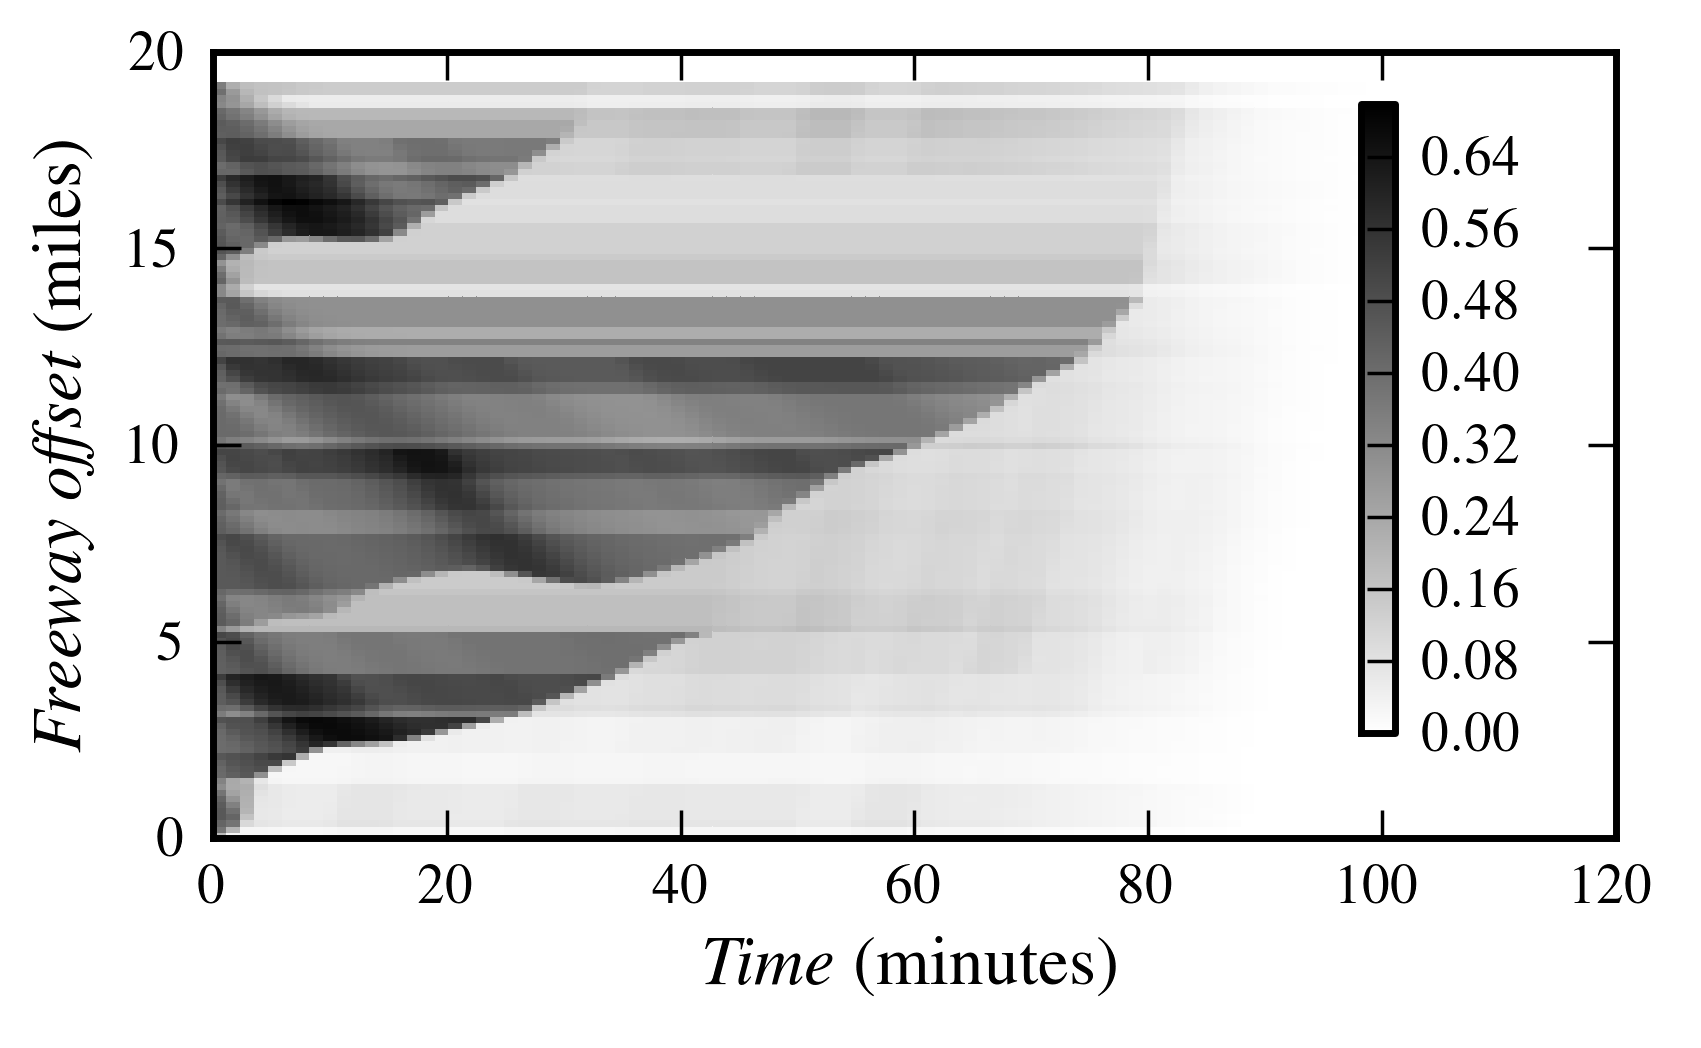
\includegraphics[width=0.45\columnwidth]{images/ncdensity}

}\hfill{}\subfloat[Onramp queue profile in units of vehicles. The onramps are only present
at certain junctions, thus why the nonzero queue lengths are sparse
in this diagram.\label{fig:Density-profile.-2}]{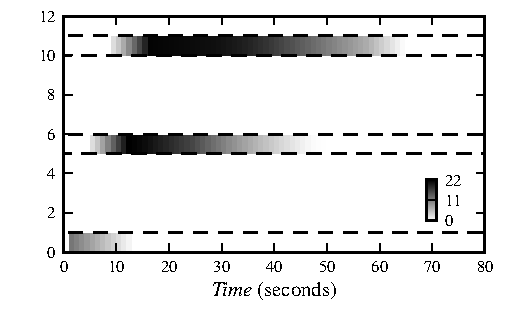
\includegraphics[width=0.45\columnwidth]{images/ncqueue}

}

\caption{Density and queue profile of no-control freeway simulation. In the
first 80 minutes, congestion pockets form on the freeway and queues
form on the onramps, then eventually clear out before 120 minutes.\label{fig:Density-and-queue}}
\end{figure}



\subsection{Finite-horizon optimal control\label{sub:Finite-horizon-optimal-control}}


\paragraph{Experimental setup}

The adjoint ramp metering algorithm is compared to the reactive Alinea
scheme, where we assume perfect boundary conditions and initial conditions
are available. The actual cost used to compare the performances of
the different methods is \emph{delay}, or the total travel time minus
the free-flow total travel time. The free-flow total travel time is
computed by assuming the critical density is infinite for all links,
thus no backwards moving congestion results from high density. The
delay gives an indication of how much improvement is possible, given
that total travel time cannot be zero at optimum.


\paragraph{Results}

\begin{figure}
\subfloat[Density difference profile in units of vehicles per mile.\label{fig:long-sim-density}]{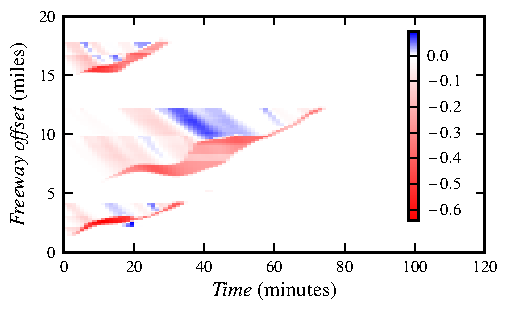
\includegraphics[width=0.45\columnwidth]{images/densdiff}

}\hfill{}\subfloat[Queue difference profile in units of vehicles.\label{fig:long-sim-queue}]{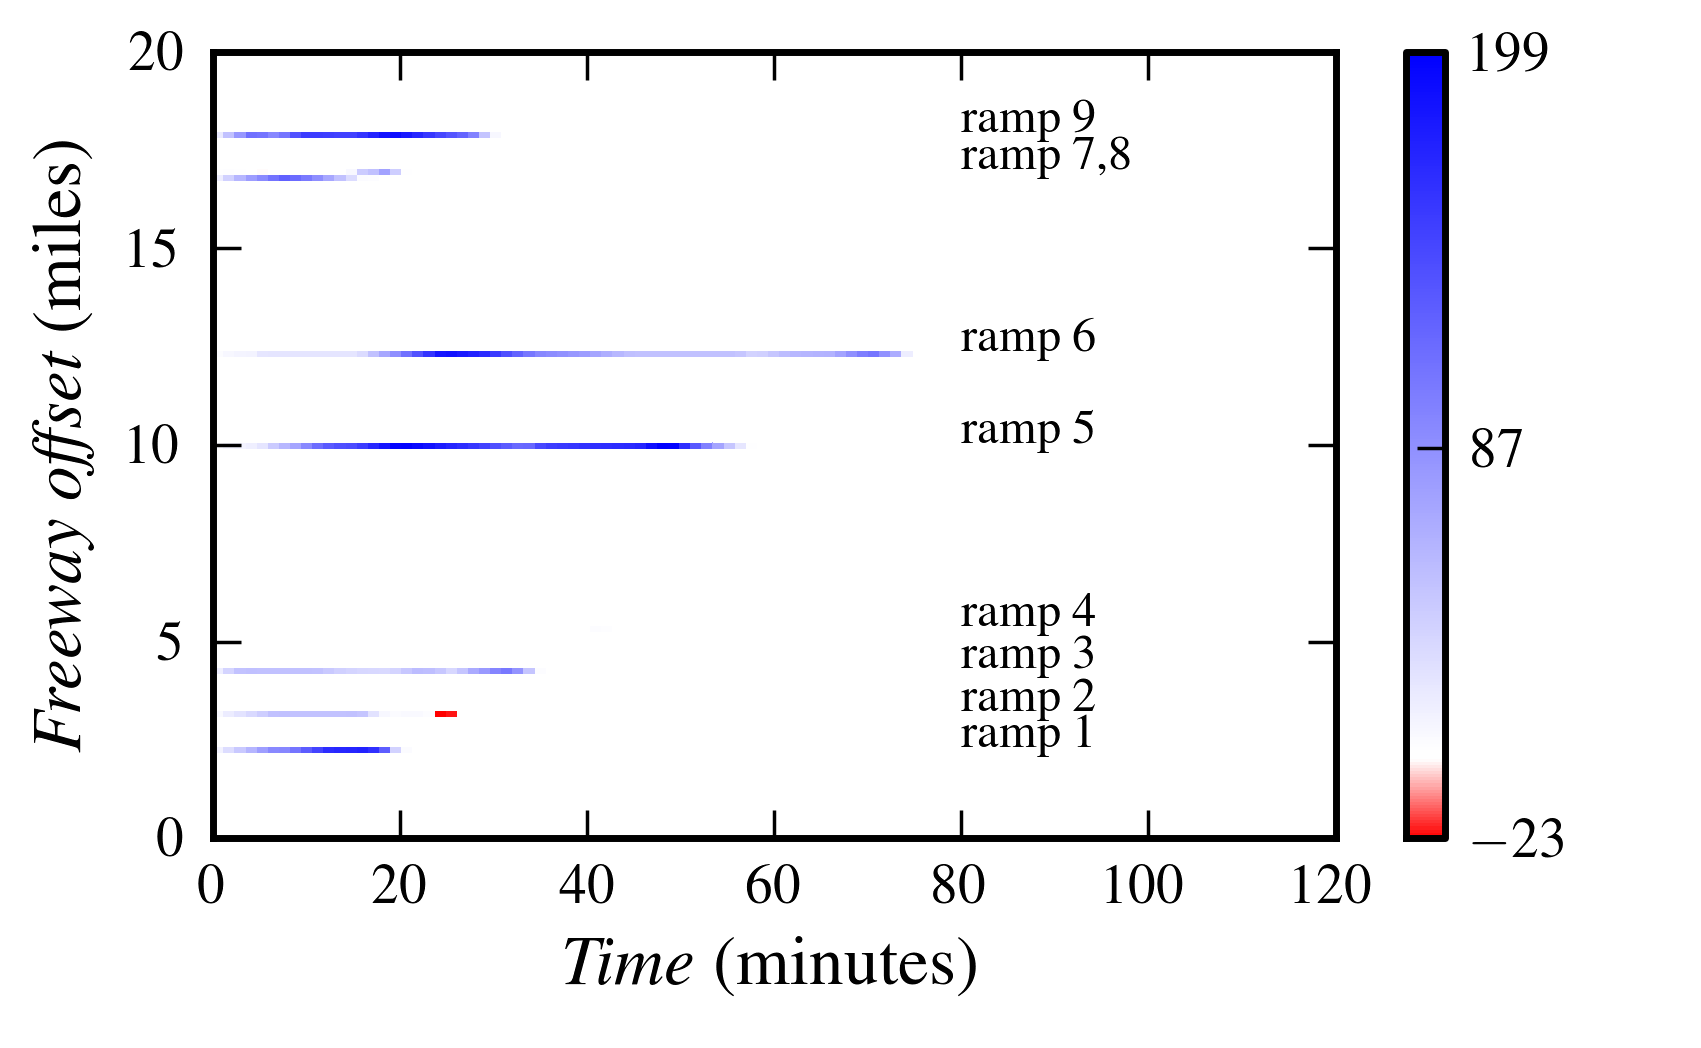
\includegraphics[width=0.45\columnwidth]{images/queuediff}

}

\caption{Profile differences for mainline densities and onramp queues. Evidenced
by the mainly negative differences in the mainline densities and the
mainly positive differences in the onramp queue lengths, the adjoint
ramp metering algorithm effectively limits onramp flows in order to
reduce mainly congestion.\label{fig:long-sim}}
\end{figure}


Figure~\ref{fig:long-sim} shows a difference profile between the
no control simulation and the simulation applying the ramp metering
policy generated from the adjoint method. Negative differences in
Figures~\ref{fig:long-sim-density} and~\ref{fig:long-sim-queue}
indicate where the adjoint method resulted in fewer vehicles for the
specific link and time-step. The adjoint method was successful in
intelligently deciding which ramps should be metered in order to improve
throughput for the mainline.
\begin{figure}
\begin{centering}
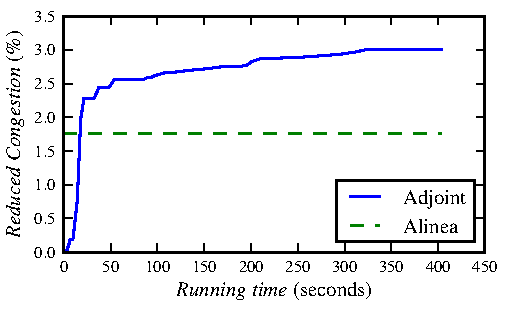
\includegraphics[width=0.65\columnwidth]{images/longsim}
\par\end{centering}

\caption{Performance versus simulation time for freeway network. The results
indicate that the algorithm can run with performance better than Alinea
if given an update time around 15 minutes.}
\end{figure}


Running time analysis shows that the adjoint method can produce beneficial
results running in real time. After just a few gradient steps, the
adjoint method outperforms the Alinea method. Given that the time
horizon of two hours is longer than the period of time one can expect
reasonable estimates of boundary conditions, more practical simulations
with shorter time horizons should permit more gradient steps in a
real-time setting.

While the queue length contains a considerable number of cars in some
onramps for the adjoint method, this problem can be accounted for
by introducing barrier terms into the cost function that limit the
maximum queue length. The Alinea method tested for the I15 network
had no prescribed maximum queue lengths as well, but was not able
to produce significant improvements, while the adjoint method was
more successful in optimizing the road network under the set of constraints.


\subsection{Model predictive control\label{sub:Model-predictive-control}}

To study the performance of the algorithm under noisy input data,
we embed both our adjoint ramp metering algorithm and the Alinea algorithm
inside of a \emph{Model predictive control }(MPC) loop.


\paragraph{Experimental setup}

The MPC loop begins at a time $t$ by estimating the initial conditions
of the traffic on the freeway network and the predicted boundary fluxes
over a certain time horizon $T_{h}$. These values are noisy, as exact
estimation of these parameters is not possible on real freeway networks.
The estimated conditions are then passed to the ramp metering algorithm
to compute an optimal control policy over the $T_{h}$ time period.
The system is then forward simulated over an update period of $T_{u}\le T_{h}$,
using the exact initial conditions and boundary conditions, as opposed
to the noisy data used to compute control parameters. The state of
the system and boundary conditions at $t+T_{u}$ are then estimated
(with noise) and the process is repeated.

A non-negative\emph{ noise factor} is used to study how the adjoint
method and Alinea perform as the quality of estimated data decreases.
The noise factor can be summarized as follows:

\[
\bar{\discrete{}{}}=\discrete{}{}*(1+noise\_factor*R)
\]


where $R$ is a uniformly distributed random variable with mean $0$
and domain $\left[-0.5,0.5\right]$. The noise factor was applied
to both initial and boundary conditions.

Two different experiments were conducted:
\begin{enumerate}
\item \textbf{Real-time I15 South}: MPC is run for the I15 South network
with $T_{h}=27$ minutes and $T_{u}=14$ minutes. A noise factor of
2\% was chosen for the initial and boundary conditions. The number
of iterations was chosen in order to ensure that each MPC iteration
finished in the pre-determined update time $T_{u}$.
\item \textbf{Noise Robustness}: MPC is for over a synthetic network with
length 5 miles and boundary conditions over 50 minutes. The experiments
are run over a profile of noise factors between 1\% and 200\%.
\end{enumerate}

\paragraph{Results}


\subparagraph{Real-time I15 South}

The results are summarized in Figure~\ref{fig:MPC-performance-on}.
The adjoint method applied once to the entire horizon with perfect
boundary and initial condition information serves as a baseline performance
for the other simulations, which had noisy input data and limited
knowledge of predicted boundary conditions. The adjoint method still
performs well under the more realistic conditions of the MPC loop
with noise, resulting in 75\% delay as compared to the no control
scenario as compared to the 71\% delay achieved by the perfect-knowledge
adjoint control. Alinea performed worse than adjoint method, only
achieving a 95\% delay as compared to no control. The results indicate
that under a realistic assumption of a 2\% noise factor in the sensor
information, the ability to consider boundary conditions in producing
ramp metering policies as an improvement upon strictly reactive policies,
such as Alinea.

\begin{figure}
\subfloat[MPC performance on I15 South network.\label{fig:MPC-performance-on}]{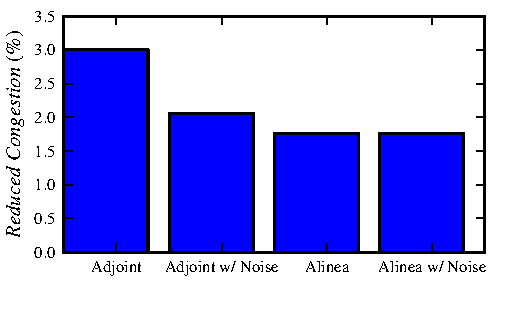
\includegraphics[width=0.45\columnwidth]{images/longmpc}

}\hfill{}\subfloat[MPC performance with increasing sensor noise.\label{fig:Ramp-metering-performance-1}]{\includegraphics[width=0.45\columnwidth]{images/noiseplot}

}
\end{figure}



\subparagraph{Noise Robustness}

Simulation results on the synthetic network with varying levels of
noise are shown in Figure~\ref{fig:Ramp-metering-performance-1}.
The adjoint method is able to outperform the Alinea method when the
noise level is less than 80\%, a reasonable assumption for data provided
by well-maintained loop detectors. As the initial and boundary condition
data deteriorates, the adjoint method becomes useless. Since Alinea
does not rely on boundary data, it is able to produce improvements,
even with severely noisy data. The results indicate that the adjoint
method will outperform Alinea under reasonable noise levels in the
sensor data.


% section numerical_results (end)

\section{Evaluation}\label{sec:evaluation}
%!TEX root =article.tex


\section{Conclusions}\label{sec:conclusions}
%!TEX root =restart.tex
\section{Conclusions\label{sec:Conclusions}}

This article has detailed a simple framework for finite-horizon optimal control 
methods on a network of scalar conservation laws derived from first 
discretizing the network via the Godunov method, then applying the discrete 
adjoint to this system. To tailor the framework to a specific application, one 
need only provide the partial derivatives of the Riemann solver at a network 
junction as well as the partial derivates of the objective. Furthermore, we 
show that for this class of problems, the sparsity pattern allows the problem 
to be implemented with only linear memory and linear computational complexity 
with respect to the number of state and control parameters. We demonstrate the 
scalability of the approach by implementing a coordinated ramp metering 
algorithm using the adjoint method and applying the algorithm to the I-15 South freeway in California. The algorithm runs in a fraction of real-time 
and produces significant improvements over existing algorithms. The ramp metering algorithm has been fully implemented within Connected Corridors~\cite{CC} system, a project by UC Berkeley and PATH for integrated corridor management, as a component of the traffic simulator module. Future work 
includes investigating decentralized, coordinated control schemes over physical 
networks via the adjoint method to allow traffic control strategies to scale to 
regional-scale networks.


%ACKNOWLEDGMENTS are optional
% \section{Acknowledgments}
% ack
\bibliographystyle{plain}
\bibliography{bib}

%!TEX root =article.tex
\appendix
%Appendix A
%\section{Appendices}
%The rules about hierarchical headings discussed above for
%the body of the article are different in the appendices.
%In the \textbf{appendix} environment, the command
%\textbf{section} is used to
%indicate the start of each Appendix, with alphabetic order
%designation (i.e. the first is A, the second B, etc.) and
%a title (if you include one).  So, if you need
%hierarchical structure
%\textit{within} an Appendix, start with \textbf{subsection} as the
%highest level. Here is an outline of the body of this
%document in Appendix-appropriate form:
%\subsection{Introduction}
%\subsection{The Body of the Paper}
%\subsubsection{Type Changes and  Special Characters}
%\subsubsection{Math Equations}
%\paragraph{Inline (In-text) Equations}
%\paragraph{Display Equations}
%\subsubsection{Citations}
%\subsubsection{Tables}
%\subsubsection{Figures}
%\subsubsection{Theorem-like Constructs}
%\subsubsection*{A Caveat for the \TeX\ Expert}
%\subsection{Conclusions}
%\subsection{Acknowledgments}
%\subsection{Additional Authors}
%This section is inserted by \LaTeX; you do not insert it.
%You just add the names and information in the
%\texttt{{\char'134}additionalauthors} command at the start
%of the document.
% \balancecolumns
% That's all folks!
\end{document}
